\setcounter{ExampleCounter}{1}
The definition of a set is a very simple one:
\paragraph{Definition:} A \textbf{set} is a collection of objects.\\

The fact that this definition is so simple is important; the simplicity is what allows us to apply the ideas of set theory to so many different fields, because we only have to be working with ``objects.''\footnote{In fact, the objects in a set could be sets themselves, so we can construct a set of sets, and so on.}

As far as notation, we use curly braces to enclose the objects in a set, called the \textbf{elements} of the set, and we separate the elements with commas.  Thus, the set that consists of the numbers 1, 2, and 3 would be written
\[S = \{1, 2, 3\}.\]

Also, based on the definition above, all it takes to define a set is to describe what objects are in it, and \textbf{the order in which they are listed is irrelevant}.  Thus, the following two sets are identical:
\[A = \{a, b, c\} \ \ \textrm{ and } \ \ B = \{b, c, a\}\]

This way of describing a set by listing its elements is often called \textbf{roster notation}.

\begin{example}{Set Notation}
Let $S$ be the set of the days of the week.  Write this using roster notation.

\sol
We could list the days of the week in any order, but of course, there is a traditional order to them.
\[\boxed{S = \{\textrm{Sunday, Monday, Tuesday, Wednesday, Thursday, Friday, Saturday}}\}\]
\end{example}

\begin{example}{Set Notation}
Create a set that represents three courses that a college student may be taking.

\sol
In this case, there is no natural order.  To make an example, we'll choose the following three courses:
\[\boxed{S = \{\textrm{Introduction to Philosophy, Western Civilizations, Statistics}\}}\]
\end{example}

\begin{try}
Let $S$ be the set of the first five odd numbers.  Write $S$ using roster notation.
\end{try}

Since a set is defined solely by what elements belong to it, we need a way to describe whether something belongs to a specific set or not.  We get a new symbol to do this:
\begin{formula}{``Is an element of''}
The symbol $\in$ is read ``belongs to'' or ``is an element of.''\\

Ex: $a \in \{a, b, c\}$ can be read ``$a$ is an element of the set $\{a, b, c\}$'' or ``$a$ belongs to the set $\{a, b, c\}$''\\

Putting a stroke through it changes the meaning to ``does not belong to.''\\

Ex: $d \notin \{a, b, c\}$
\end{formula}
\vfill
\pagebreak

\begin{example}{Using Element Notation}
Place $\in$ or $\notin$ in each of the following blanks to make each statement true.\\

\begin{enumerate}[(a)]
\item Apple \line(1,0){25}\ $F$, where $F$ is the set of all fruits\\

\item $g$ \line(1,0){25}\ $\{a, e, i, o, u\}$\\

\item 3 \line(1,0){25}\ the set of positive real numbers
\end{enumerate}

\sol
It should be clear that an apple belongs to the first set, and 3 belongs to the set of positive real numbers, but $g$ does not belong to the given set of letters.\\

\begin{enumerate}[(a)]
\item Apple $\boxed{\in}$ $F$, where $F$ is the set of all fruits\\

\item $g$ $\boxed{\notin}$ $\{a, e, i, o, u\}$\\

\item 3 $\boxed{\in}$ the set of positive real numbers
\end{enumerate}
\end{example}

\subsection{Common Sets}

There are some sets that come up more than others, so we'll take a moment here to list them, along with a symbol that we can use for each.
\begin{center}
\begin{tabularx}{3.5in}{|c | X|}
\hline
& \\
$\mathbb{R}$ & The set of all real numbers; basically, any number that you can use to count or measure something\footnote{Notice that we can't list this set like we do the others, because there's no way to account for all of them.}\\
& \\
\hline
& \\
$\mathbb{Z}$ & The integers\footnote{The letter Z comes from the German word for ``number.''}\footnote{The ellipses ($\ldots$) indicate that this is an infinite set, extending forever in both directions.}: $\{\ldots, -3,-2,-1,0,1,2,3, \ldots\}$\\
& \\
\hline
& \\
$\mathbb{N}$ & The natural numbers (or counting numbers)\footnote{These are the positive integers.}: $\{1,2,3,\ldots\}$\\
& \\
\hline
\end{tabularx}
\end{center}

These symbols, along with the element symbol, give us another way to define sets, using what is sometimes called \textbf{set-builder notation}, where instead of listing the elements of a set, we give a rule that defines them.

For instance, we could write \[S = \{x \in \mathbb{N}\ \ |\ x \textrm{ is even}\}.\]  If we wanted to read it, we would need to know that the vertical line in the middle of the set is read ``such that,'' so the line above would read 
\begin{center}
``$S$ is the set of all $x$ in the natural numbers \textbf{such that} $x$ is even''
\end{center}
and if we started listing elements of this set, we would write \[S = \{2, 4, 6, 8, 10, \ldots\}.\]  Notice that we have to use ellipses when we write it this way, to denote that this set keeps on going and going.  By writing it in set-builder notation, though, we have a concise way of accounting for all the elements of the set by giving the rule that they all have to satisfy.
\pagebreak
\text{}
\vfill

We do this naturally in language; we might talk about the set of all sophomores at a college, or the set of people on the Dean's List.  Remember, to define a set, all we need is a clear indication of what elements belong to a set; we can do this by listing them, or by giving a rule that they all must follow.
\vfill

\begin{example}{Set Builder Notation}
List the elements of the following sets that are described using set builder notation.  If the sets are infinite, list the first five elements.
\begin{enumerate}[(a)]
\item $A = \{x \in \mathbb{Z}\ \ |\ x \geq -3\}$
\item $B = \{x \in \mathbb{N}\ \ |\ 2 \leq x \leq 8\}$
\end{enumerate}

\sol
\begin{enumerate}[(a)]
\item $A = \{x \in \mathbb{Z}\ \ |\ x \geq -3\}$
\[\boxed{A = \{-3, -2, -1, 0, 1, \ldots\}}\]

\item $B = \{x \in \mathbb{N}\ \ |\ 2 \leq x \leq 8\}$
\[\boxed{B = \{2, 3, 4, 5, 6, 7, 8\}}\]
\end{enumerate}
\end{example}
\vfill

\begin{try}
Find a way to write the following set in set builder notation.
\[C = \{\ldots, 3, 4, 5, 6, 7\}\]
\end{try}
\vfill

\subsection{Subsets}

The idea of a subset is an intuitive one; if I told you that your class is a subset of students at your college, you would intuitively understand what I meant.  We can make this definition more precise, though:
\vfill

\begin{formula}{Subset}
We say that one set $A$ is a \textbf{subset} of another set $B$, written \[A \subseteq B\] if every element in $A$ is also an element of $B$.\\

This notation can be informally read as ``$A$ is contained in $B$,'' which can be helpful in remembering the notation, since the subset symbol looks like a capital C.
\end{formula}
\vfill

In other words, your class is a subset of students at your college because every student in your class is also a student at your college.  However, we probably couldn't say that your friends form a subset of students at your college, because, while many of your friends may be at your school, you may have friends that do not belong to that set.
\vfill
\text{}
\vfill
\pagebreak

\begin{example}{Subsets}
Place $\subseteq$ or $\cancel{\subseteq}$ in each of the following blanks to make each statement true.\\

\begin{enumerate}[(a)]
\item $\{$Spring, Fall$\}$ \line(1,0){25}\ $\{$Winter, Spring, Summer, Fall$\}$\\

\item $\{$Green, Blue, Red$\}$ \line(1,0){25}\ $\{$Red, Yellow, Green$\}$\\

\item $\{$North, South, East, West$\}$ \line(1,0){25}\ $\{$West, South, North, East$\}$\\

\item $\{-2,5,-1\}$ \line(1,0){25}\ $\mathbb{Z}$\\

\item $\{-2,5,-1\}$ \line(1,0){25}\ $\{x \in \mathbb{Z}\ |\ x > 0\}$
\end{enumerate}

\sol
\begin{enumerate}[(a)]
\item $\{$Spring, Fall$\}$ $\boxed{\subseteq}$ $\{$Winter, Spring, Summer, Fall$\}$, because both elements in the first set also appear in the second set.\\

\item $\{$Green, Blue, Red$\}$ $\boxed{\cancel{\subseteq}}$ $\{$Red, Yellow, Green$\}$, because the element ``Blue'' appears in the first set, but not the second one.\\

\item $\{$North, South, East, West$\}$ $\boxed{\subseteq}$ $\{$West, South, North, East$\}$, because, once again, every element in the first set also appears in the second set (they happen to be the exact same set, just written in a different order).\\

\item $\{-2,5,-1\}$ $\boxed{\subseteq}$ $\mathbb{Z}$, because each of those numbers in the first set are integers.\\

\item $\{-2,5,-1\}$ $\boxed{\cancel{\subseteq}}$ $\{x \in \mathbb{Z}\ |\ x > 0\}$, because not all of the numbers in the first set meet the condition in the second set (two of them are negative).
\end{enumerate}
\end{example}

\begin{try}[http://hartleymath.com/versatilemath/tryit/\#/set-theory--subset-notation]
Place $\subseteq$ or $\cancel{\subseteq}$ in each of the following blanks to make each statement true.\\

\begin{enumerate}[(a)]
\item $\{$1,7,6,3$\}$ \line(1,0){25}\ $\{x \in \mathbb{N} | 1 \leq x \leq 10\}$\\

\item $\{$a, b, c$\}$ \line(1,0){25}\ $\{$a, e, i, o, u$\}$
\end{enumerate}
\end{try}

Notice in the third item of the example above that the given set was contained in itself.  This will always be true by definition: naturally, every element in $A$ will be an element in $A$, so \[A \subseteq A.\]  That is why we include a line below the C, similar to how we use the symbol $\leq$ to indicate ``less than \textbf{or} equal to.''  The subset symbol can be thought of as ``is contained in \textbf{or} equal to.''

Therefore, we can also define a \textbf{proper subset}, which is a subset that is \textbf{not} equal to the set that contains it.  This is written without the line underneath the C.

For instance, $\{1,2,3\}$ is a proper subset of $\{1,2,3,4\}$, but $\{1,2,3,4\}$ is not.  In general,
\[A \subset B\] if $A$ is completely contained in $B$, and $B$ has at least one extra element that $A$ doesn't have.
\pagebreak

\begin{example}{Proper Subsets}
Place $\subset$ or $\cancel{\subset}$ in each of the following blanks to make each statement true.\\

\begin{enumerate}[(a)]
\item $\{0,1,2\}$ \line(1,0){25}\ $\mathbb{Z}$\\

\item $\{0,1,2\}$ \line(1,0){25}\ $\{x \in \mathbb{Z} \ | \ 0 \leq x \leq 2\}$
\end{enumerate}

\sol
\begin{enumerate}[(a)]
\item $\{0,1,2\}$ $\boxed{\subset}$ $\mathbb{Z}$, because every element in the first set belongs to the set of integers, $\mathbb{Z}$.\\

\item $\{0,1,2\}$ $\boxed{\cancel{\subset}}$ $\{x \in \mathbb{Z} \ | \ 0 \leq x \leq 2\}$, because the two sets are equal, so the first set is not a \emph{proper} subset of the second.
\end{enumerate}
\end{example}

Of course, a given set could be a subset (or proper subset) of many different sets.  For instance, consider the set $A = \{$``Much Ado About Nothing'', ``MacBeth'', ``A
Midsummer's Night Dream''$\}$.  This is a subset of the set of William Shakespeare's plays, which of course is itself a subset of all plays and all British literature, as shown in the \textbf{Venn diagram} below (we'll see more of these diagrams in the next section).

\begin{center}
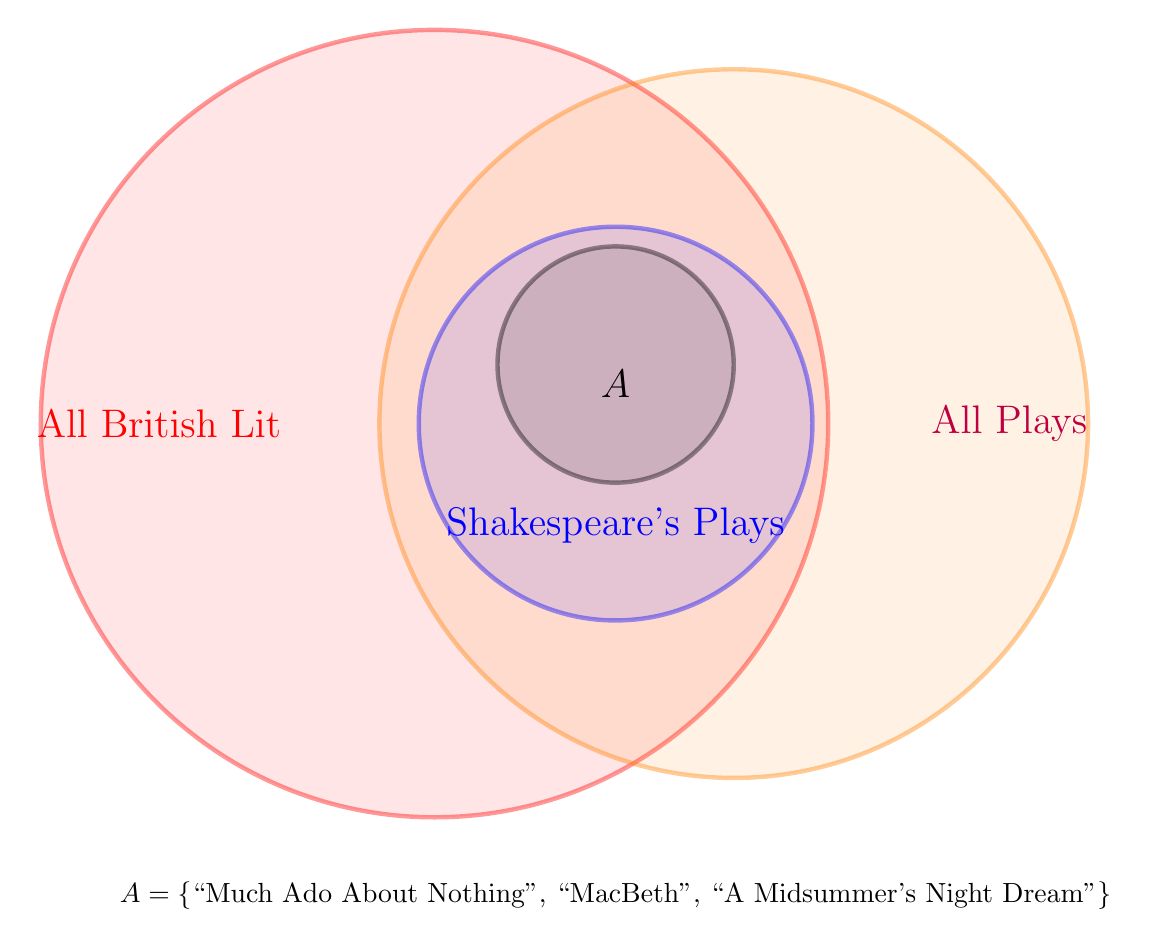
\begin{tikzpicture}
  \draw [ultra thick,color=red, fill=red,draw opacity=0.4, fill opacity=0.1] (-2.3,0) circle (5cm);
  \draw [ultra thick,color=orange, fill=orange,draw opacity=0.4, fill opacity=0.1] (1.5,0) circle (4.5cm);
  \draw [ultra thick,color=blue, fill=blue,draw opacity=0.4, fill opacity=0.1] (0,0) circle (2.5cm);
  \draw [ultra thick,color=black, fill=black,draw opacity=0.4, fill opacity=0.1] (0,0.75) circle (1.5cm);
  
  
  \draw [yshift=0.5cm,xshift=0cm] node {\color{black}\Large $A$};
  \draw [yshift=-1.3cm,xshift=0cm] node {\color{blue}\Large Shakespeare's Plays};
  \draw [yshift=0cm,xshift=-5.8cm] node {\color{red}\Large All British Lit};
  \draw [yshift=0cm,xshift=5cm] node {\color{purple}\Large All Plays};
  \draw [yshift=-6cm,xshift=0cm] node {\color{black} $A = \{$``Much Ado About Nothing'', ``MacBeth'', ``A
Midsummer's Night Dream''$\}$};
\end{tikzpicture}
\end{center}
\pagebreak

\subsection{The Empty Set}
What if we describe a set like the following?
\[\{x \in \mathbb{R}\ |\ x < 2 \textrm{ and } x > 5\}\]
If you try to list the elements in this set, you'll quickly find that there are none, because it is impossible for a number to be simultaneously less than 2 and greater than 5.

This is an example of one way to describe the \textbf{empty set}\footnote{Note that we call it \emph{the} empty set because every empty set is identical to every other empty set, so there's really just one distinct empty set.}, whose name gives it away: the empty set is defined as the set with no elements.

\begin{formula}{The Empty Set}
The set $\{\ \}$, which contains no elements, is called the \textbf{empty set} and is written with the symbol $\varnothing$.\\

(note: it is not written $\{\varnothing\}$, because that would mean a set with one element, and that element is the empty set)
\end{formula}

\begin{example}{Empty Set}
Which of the following sets are empty?
\begin{enumerate}[(a)]
\item The set of the days of the week whose names start with P.
\item The set of students at Frederick Community College under the age of 25.
\end{enumerate}

\sol
\begin{enumerate}[(a)]
\item This set is empty; since there are no days of the week that start with P, there are no elements in this set.
\item Since there are students that fall into this category, this set is not empty.
\end{enumerate}
\end{example}

\subsection{Cardinality}
The \textbf{cardinality} of a set is just a fancy term for the number of elements it contains.

\begin{formula}{Cardinality}
The \textbf{cardinality} of a set $A$ is the number of \emph{distinct} elements in $A$.\\

The cardinality of $A$ is denoted $n(A)$, or sometimes $|A|$.
\end{formula}

\begin{example}{Cardinality}
Find the cardinality of each of the following sets.
\begin{enumerate}[(a)]
\item $A = \{3, 5, 9, 32\}$
\item $B = \{2, 3, 2, 4, 2\}$
\item $C = \{31, 32, \ldots, 58\}$
\item $D = \varnothing$
\end{enumerate}
\pagebreak

\sol
\begin{enumerate}[(a)]
\item Since there are four elements listed, $\boxed{n(A) = 4}$.
\item There are five elements listed, but notice that 2 is listed three times, so there are really only three \emph{distinct} elements in this set.  Therefore, $\boxed{n(B) = 3}$.
\item Even though only three elements are shown, the ellipses indicate that this set includes all the integers from 31 to 58.  Since this includes 28 integers (note carefully, not 27), $\boxed{n(C) = 28}$.
\item There are no elements in the empty set, so $\boxed{n(D) = 0}$.
\end{enumerate}
\end{example}
\vfill
\text{}
\vfill

\subsection{Summary}
Since we've encountered so many new terms and symbols in this section, it may be helpful to pause for a moment and review these new concepts.
\vfill

\begin{formula}{New Terms}
\paragraph{Set} A collection of objects
\paragraph{Subset} $A$ is a subset of $B$ if all the elements of $A$ are also elements of $B$
\paragraph{Proper subset} A subset that is not equal to its containing set
\paragraph{Empty set} The set that contains no elements
\paragraph{Cardinality} The number of distinct elements in a set
\end{formula}
\vfill

\begin{formula}{New Symbols and Notation}
\paragraph{Set notation} Uses curly braces: $\{\ldots\}$
\paragraph{$\in$} Is an element of
\paragraph{$\mathbb{R}$} The set of real numbers
\paragraph{$\mathbb{Z}$} The set of integers
\paragraph{$\mathbb{N}$} The set of natural numbers (integers starting at 1)
\paragraph{$\subseteq$} Subset
\paragraph{$\subset$} Proper subset
\paragraph{$\varnothing$} The empty set
\paragraph{$n(A)$} The cardinality of $A$
\end{formula}
\vfill
\text{}
\vfill
\pagebreak

\subsection{Sidenote: Infinite Sets}
For some sets, we can count the number of elements and call that number their cardinality.  These are called \textbf{finite sets}.  Others, like the integers, for instance, are \textbf{infinite sets}.  Can we talk about the cardinality of an infinite set?

It turns out that we can.  Georg Cantor, the founder of set theory, was one of the first mathematicians to dive headfirst into an investigation of infinite sets (for which his career suffered tremendously as others ridiculed his work at the time), and his contributions have since been lauded as groundbreaking.

Let's start with the natural numbers ($\mathbb{N} = \{1,2,3,\ldots\}$), an infinite set.  The cardinality of this set is not a number, because there are infinitely many elements in the set, but we call this cardinality aleph-nought (aleph being the first character in the Hebrew alphabet), written $\aleph_0$.

Now, here comes the mind-bendy part, so hang on tight.  It makes sense to say that two sets have the same number of elements (the same cardinality) if we can place their elements in one-to-one correspondence.  In other words, if each Shark can pair up with exactly one Jet, there must be the same number of Sharks and Jets.

You may not believe this the first time you hear it, but it's true: the natural numbers and the integers have the same cardinality.  But hold on, there are clearly more integers, right, since there are negative numbers in the integers?  But look, we can place the natural numbers and the integers in a one-to-one correspondence:
\begin{center}
\begin{tabular}{c | c c c c c c c c c c c}
$\mathbb{N}$ & 1 & 2 & 3 & 4 & 5 & 6 & 7 & 8 & 9 & 10 & $\ldots$\\
& & & & & & & & & & & \\
& $\updownarrow$ & $\updownarrow$ & $\updownarrow$ & $\updownarrow$ & $\updownarrow$ & $\updownarrow$ & $\updownarrow$ & $\updownarrow$ & $\updownarrow$ & $\updownarrow$ & \\
& & & & & & & & & & & \\
$\mathbb{Z}$ & 0 & 1 & $-1$ & 2 & $-2$ & 3 & $-3$ & 4 & $-4$ & 5 & $\ldots$
\end{tabular}
\end{center}

If you think that's \textbf{at all} interesting, Google ``Hilbert's Hotel'' and enjoy.\\

Any infinite set that is infinite in this same way, meaning that it can be placed in one-to-one correspondence with the natural numbers, is called a \textbf{countable} set.  There are some infinite sets that are uncountable; the set of real numbers is the notable example of this.  There is no way to count through the real numbers and make any progress, unlike the way that we can count through the natural numbers or the integers.\\
\vfill
\pagebreak

\begin{proc}{Russell's Paradox}
Since\marginnote{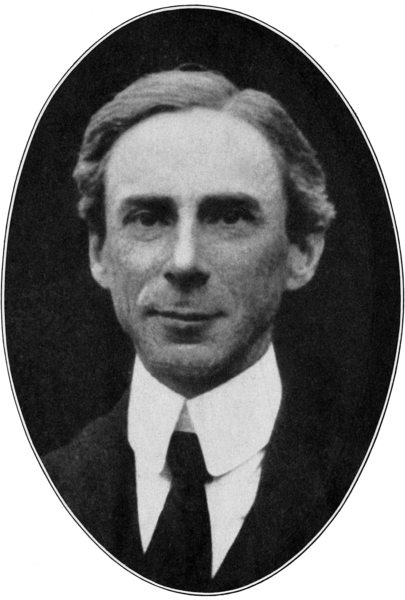
\includegraphics[width=1.3in]{Bertrand_Russell}\\ Bertrand Russell in 1916} the definition of a set is so broad, we can in theory define a set of sets.  For instance, you could treat every baseball team in the MLB as a set, where the elements are the players on that team, and then the MLB could be a set of sets, where its elements are the teams in the league.\\

However, a subtle problem arises here, and Russell's Paradox, discovered by Bertrand Russell in 1901, is a famous illustration of it.\\

Before we state this paradox, we'll give two informal representations of it.\\

\paragraph{Barber Paradox} Suppose in a certain town, there is a barber who shaves all men who don't shave themselves, and these are the only men he shaves.  Does he shave himself?\\

Of course, if he doesn't shave himself, he is one of the ones in the category of people that he does shave, and if he does shave himself, he is not, leading to a contradiction.\\

\paragraph{Library Paradox} Consider another situation: there are 100 libraries in a country, and each library has a book that is a written catalog of all the books in that library.  As each library is compiling its catalog, they face this question: should they list this catalog as one of the books in the library?  Fifty of the libraries choose to list their catalog \emph{in} their catalog, and 50 choose not to.\\

Now, suppose the national library wants to create a master catalog of all these individual catalogs.  In fact, they create two lists: one is the list of all the catalogs that list themselves, and the other is the list of those that don't.

Here comes the paradox: should this master catalog list itself in the category of those that don't?  If it lists itself in that category, it no longer belongs to that category, and vice versa.\\

\paragraph{Russell's Paradox} Russell's Paradox, in precise terms, goes like this: let $R$ be the set of all sets that are not members of themselves.  If $R$ is a member of itself, then by definition, it cannot be a member of itself, and vice versa.  Symbolically, we could write it this way:
\[R = \{x\ |\ x \notin x\} \ \ \textrm{implies}\ \ R \in R \textrm{ if and only if } R \notin R\]

\paragraph{Solution} This paradox may seem abstract and a little contrived, but it was a powerful blow to the development of set theory, because it struck at the heart of what it means to define a set.\\

To resolve this paradox, the generally accepted set theory (Zermelo-Fraenkel) essentially did away with the ability to define sets the way that Russell did, requiring sets to be \textbf{well-defined}.
\end{proc}